\documentclass[12pt,letterpaper]{article}

\usepackage{amsmath, amsthm, amsfonts, amssymb}
\usepackage{microtype, parskip, graphicx}
\usepackage[comma,numbers,sort&compress]{natbib}
\usepackage{lineno}
\usepackage{longtable}
\usepackage{docmute}
\usepackage{caption, subcaption, multirow, morefloats, rotating}
\usepackage{wrapfig}
\usepackage{hyperref}

\frenchspacing

\begin{document}
\section*{Materials and Methods}

\subsection*{Taxon occurrences and species-level information}
All fossil occurrence information used in this analysis was downloaded from the Paleobiology Database (PBDB). The initial download restricted occurrences to Mammalia observed in North America between the Maastrichtian (72-66 Mya) and Gelasian (2.58-1.8 Mya) stages \citep{Cohen2015}. Taxonomic, stratigraphic, and ecological metadata for each occurrence and species was also downloaded. A new download for a raw, unfiltered PBDB datafile following the same criterion used here is available at \url{http://goo.gl/2slgeU}. The raw datafile used as a part of this study, along with all code for filtering, manipulating, and modeling is available at \url{http://github.com/psmits/coping}.
%https://paleobiodb.org/data1.2/occs/list.csv?datainfo&rowcount&base_name=Mammalia&taxon_reso=species&interval=Maastrichtian,Gelasian&cc=NOA&show=class,genus,ecospace,loc,strat,stratext,lith,acconly. 

After being downloaded, the raw occurrence data was then sorted, cleaned, and manipulated programmatically before analysis. Occurrences were restricted to those occurring between 64 and 2 million years ago (Mya); this age restriction was to insure that observation time series lines up with the temperature time series described below \citep{Cramer2011}. All taxa whose life habit was classified as either volant (e.g. Chiroptera) or aquatic (e.g. Cetacea) were excluded from this analysis because of their lack of direct applicability to the study of terrestrial species pools.

Many species taxonomic assignments as present in the raw PBDB data were updated for accuracy and consistency. Species present in the PBDB have some taxonomic information, including possible Family and Order assignments. In order to increase consistency between species and reflect more recent taxonomic assignments, each species taxonomic assignments updated as follows: 1) species family and order assignemnts as present in the Encyclopedia of life (\url{http://eol.org}) was downloaded using the \textit{taxize} package for R CITATION; 2) for species not present in the EoL or not assigned order, their taxonomic inforation was further updated based on whatever family information was recorded in the PBDB or EoL; 3) for species still missing order assignemnts, their genus information was used to assign either an order or family, which was then used to assign an order. This procedure is similar to that used in \citet{Smits2015b} and is detailed in the code repository associated with this study.
% i actually do a lot of swapping and fixing in this step. might want to better explain it
% PBDB forms basis
% grab from EoL
%   replace family and order to match EoL
% for things not in EoL
%   some PBDB things have family but no order
%   i've made a cypher for families in order
%   update using cypher
% some orders need changing
% sometimes families are treated as orders and need fixing
%   i've written code for that too
%  
% flow chart figure for supplement


Species functional group is defined as the combination of locomotor and diet categories; the goal is to classify species based on the manner with which they interact with their environment. Mammal species records in the PBDB have life habit (i.e. locomotor category) and dietary category assignments. In order to simplify interpretation, analysis, and per-functional group sample size these classifications were coarsened in a similar manner to \citet{Smits2015b} (Table \ref{tab:trait_cats}). Ground dwelling species locomotor categories were then reassigned based on the ankle posture associated with their taxonomic group, as described in Table \ref{tab:posture} \citep{Carrano1999}. Ankle posture was assumed uniform for all species within a taxonomic group except for those species assigned a non-ground dwelling locomotor category in the PBDB, which retained their non-ground dwelling assignment. All species for which it was possible to assign a locomotor category had one assigned, including species for which post-crania are unknown but for which a taxonomic grouping is known. Ground dwelling species which were unable to be reassigned based on ankle posture were excluded from analysis. Finally, ecotype categories with less than 10 total species were excluded, yielding a total of 18 observed ecotypes out of a possible 24.

\begin{table}[ht]
  \centering
  \caption{Species trait assignments in this study are a coarser version of the information available in the PBDB. Information was coarsened to improve per category sample size. Assignments are considered uniform within that taxonomic group unless there is a non-ground dwelling assignment for a species in the PBDB.}
  \begin{tabular}[ht]{ l | l | l }
    \hline
    \multicolumn{2}{ c |}{This study} & PBDB categories \\
    \hline
    \multirow{4}{*}{Diet} & Carnivore & Carnivore \\
    & Herbivore & Browser, folivore, granivore, grazer, herbivore. \\
    & Insectivore & Insectivore. \\
    & Omnivore & Frugivore, omnivore. \\ 
    \hline
    \multirow{3}{*}{Locomotor} & Arboreal & Arboreal.\\
    & Ground dwelling & Fossorial, ground dwelling, semifossorial, saltatorial. \\
    & Scansorial & Scansorial. \\
    \hline
  \end{tabular}
  \label{tab:trait_cats}
\end{table}


\begin{center}
  \begin{longtable}{ l l l }
    \caption[Posture assignment based on taxonomy]{Posture assignment based on taxonomy} \label{tab:posture} \\

    Order & Family & Stance \\ \hline
    \endfirsthead
  
    \multicolumn{3}{p{\textwidth}}{{ \bfseries \tablename\ \thetable{} -- continued from previous page}} \\
    \hline Order & Family & Stance \\ \hline
    \endhead
      
    \hline \multicolumn{3}{p{\textwidth}}{{Continued on next page}} \\ \hline
    \endfoot
  
    \hline \hline
    \endlastfoot
  
    & Ailuridae & plantigrade \\ 
    & Allomyidae & plantigrade \\ 
    & Amphicyonidae & plantigrade \\ 
    & Amphilemuridae & plantigrade \\ 
    & Anthracotheriidae & digitigrade \\ 
    & Antilocapridae & unguligrade \\ 
    & Apheliscidae & plantigrade \\ 
    & Aplodontidae & plantigrade \\ 
    & Apternodontidae & scansorial \\ 
    & Arctocyonidae & unguligrade \\ 
    & Barbourofelidae & digitigrade \\ 
    & Barylambdidae & plantigrade \\ 
    & Bovidae & unguligrade \\ 
    & Camelidae & unguligrade \\ 
    & Canidae & digitigrade \\ 
    & Cervidae & unguligrade \\ 
    & Cimolodontidae & scansorial \\ 
    & Coryphodontidae & plantigrade \\ 
    & Cricetidae & plantigrade \\ 
    & Cylindrodontidae & plantigrade \\ 
    & Cyriacotheriidae & plantigrade \\ 
    & Dichobunidae & unguligrade \\ 
    Dinocerata &  & unguligrade \\ 
    & Dipodidae & digitigrade \\ 
    & Elephantidae & digitigrade \\ 
    & Entelodontidae & unguligrade \\ 
    & Eomyidae & plantigrade \\ 
    & Erethizontidae & plantigrade \\ 
    & Erinaceidae & plantigrade \\ 
    & Esthonychidae & plantigrade \\ 
    & Eutypomyidae & plantigrade \\ 
    & Felidae & digitigrade \\ 
    & Florentiamyidae & plantigrade \\ 
    & Gelocidae & unguligrade \\ 
    & Geolabididae & plantigrade \\ 
    & Glyptodontidae & plantigrade \\ 
    & Gomphotheriidae & unguligrade \\ 
    & Hapalodectidae & plantigrade \\ 
    & Heteromyidae & digitigrade \\ 
    & Hyaenidae & digitigrade \\ 
    & Hyaenodontidae & digitigrade \\ 
    & Hypertragulidae & unguligrade \\ 
    & Ischyromyidae & plantigrade \\ 
    & Jimomyidae & plantigrade \\ 
    Lagomorpha &  & digitigrade \\ 
    & Leptictidae & plantigrade \\ 
    & Leptochoeridae & unguligrade \\ 
    & Leptomerycidae & unguligrade \\ 
    & Mammutidae & unguligrade \\ 
    & Megalonychidae & plantigrade \\ 
    & Megatheriidae & plantigrade \\ 
    & Mephitidae & plantigrade \\ 
    & Merycoidodontidae & digitigrade \\ 
    Mesonychia &  & unguligrade \\ 
    & Mesonychidae & digitigrade \\ 
    & Micropternodontidae & plantigrade \\ 
    & Mixodectidae & plantigrade \\ 
    & Moschidae & unguligrade \\ 
    & Muridae & plantigrade \\ 
    & Mustelidae & plantigrade \\ 
    & Mylagaulidae & fossorial \\ 
    & Mylodontidae & plantigrade \\ 
    & Nimravidae & digitigrade \\ 
    & Nothrotheriidae & plantigrade \\ 
    Notoungulata &  & unguligrade \\ 
    & Oromerycidae & unguligrade \\ 
    & Oxyaenidae & digitigrade \\ 
    & Palaeomerycidae & unguligrade \\ 
    & Palaeoryctidae & plantigrade \\ 
    & Pampatheriidae & plantigrade \\ 
    & Pantolambdidae & plantigrade \\ 
    & Periptychidae & digitigrade \\ 
    Perissodactyla &  & unguligrade \\ 
    & Phenacodontidae & unguligrade \\ 
    Primates &  & plantigrade \\ 
    & Procyonidae & plantigrade \\ 
    & Proscalopidae & plantigrade \\ 
    & Protoceratidae & unguligrade \\ 
    & Reithroparamyidae & plantigrade \\ 
    & Sciuravidae & plantigrade \\ 
    & Sciuridae & plantigrade \\ 
    & Simimyidae & plantigrade \\ 
    & Soricidae & plantigrade \\ 
    & Suidae & digitigrade \\ 
    & Talpidae & fossorial \\ 
    & Tayassuidae & unguligrade \\ 
    & Tenrecidae & plantigrade \\ 
    & Titanoideidae & plantigrade \\ 
    & Ursidae & plantigrade \\ 
    & Viverravidae & plantigrade \\ 
    & Zapodidae & plantigrade \\ 
    \hline
  \end{longtable}
\end{center}


Estimates of species mass used in this study were sourced from multiple databases and papers, especially those focusing on similar macroevolutionary or macrecological questions \citep{Tomiya2013,Brook2004a,Freudenthal2013,McKenna2011,Raia2012f,Smith2004}; this is similar to \citet{Smits2015b}. When a species' mass was not available, proxy measures were used to estimates their mass. For example, given a measurement of a mammal tooth size, it is possible and routine to estimate its mass given some regression equation (Table \ref{tab:mass_est}). The PBDB has one or more body part measures for many species. These were used as body size proxies for many species, as was the case in \citet{Smits2015b}. Mass was log-transformed and then rescaled by first subtracting mean log-mass from all mass estimates, then dividing by two-times its standard deviation; this insures that the magnitude of effects for both continuous and discrete covariates are directly comparable \citep{Gelman2007,Gelman2008}.

In total, 1400 mammal species occurrence histories were included in this study after applying all of the restrictions above.

\begin{table}[ht]
  \centering
  \caption{Regression equations used in this study for estimating body size. Equations are presented with reference to taxonomic grouping, part name, and reference.}
  \begin{tabular}{l | l | l | l}
    \hline
    Group & Equation & log(Measurement) & Source \\
    \hline
    General & \(\log(m) = 1.827x + 1.81\) & lower m1 area &  \cite{Legendre1986} \\
    General & \(\log(m) = 2.9677x - 5.6712\) & mandible length & \cite{Foster2009a} \\
    General & \(\log(m) = 3.68x - 3.83\) & skull length & \cite{Luo2001} \\
    Carnivores & \(\log(m) = 2.97x + 1.681\) & lower m1 length & \cite{VanValkenburgh1990} \\
    Insectivores & \(\log(m) = 1.628x + 1.726\) & lower m1 area & \cite{Bloch1998} \\
    Insectivores & \(\log(m) = 1.714x + 0.886\) & upper M1 area & \cite{Bloch1998} \\
    Lagomorph & \(\log(m) = 2.671x - 2.671\) & lower toothrow area & \cite{Tomiya2013} \\
    Lagomorph & \(\log(m) = 4.468x - 3.002\) & lower m1 length & \cite{Tomiya2013} \\
    Marsupials & \(\log(m) = 3.284x + 1.83\) & upper M1 length & \cite{Gordon2003} \\
    Marsupials & \(\log(m) = 1.733x + 1.571\) & upper M1 area & \cite{Gordon2003} \\
    Rodentia & \(\log(m) = 1.767x + 2.172\) & lower m1 area & \cite{Legendre1986} \\
    Ungulates & \(\log(m) = 1.516x + 3.757\) & lower m1 area & \cite{Mendoza2006} \\
    Ungulates & \(\log(m) = 3.076x + 2.366\) & lower m2 length & \cite{Mendoza2006} \\
    Ungulates & \(\log(m) = 1.518x + 2.792\) & lower m2 area & \cite{Mendoza2006} \\
    Ungulates & \(\log(m) = 3.113x - 1.374\) & lower toothrow length & \cite{Mendoza2006} \\
    \hline
  \end{tabular}
  \label{tab:mass_est}
\end{table}


All fossil occurrences from 64 to 2 million years ago (Mya) were binned into the 18 North American Land Mammal Ages (NALMA) covered by this interval CITATION. The choice of binning by NALMA reflects the belief that these represent distinct communities or periods of mammal evolution, something that is central to this study. The NALMA units in this study are listed in Table \ref{tab:nalma}. %Additionally, because of the inherently discrete nature of the fossil record it can be hard to re-bin fossils by temporal interval because of the inherent uncertainty in their ages CITATION.

\begin{table}[ht]
  \centering
  \caption{Listed in order from oldest to youngest NALMA.:}
  \begin{tabular} { l l }
    \hline
    NALMA & Start Age (Mya) \\
    Torrejonian & 63.3 \\
    Tiffanian & 60.2 \\
    Clarkforkian & 56.8 \\
    Wasatchian & 55.4 \\
    Bridgerian & 50.3 \\
    Uintan & 46.2 \\
    Duchesnean & 42 \\
    Chadronian & 38 \\
    Orellan & 33.9 \\
    Whitneyan & 33.3 \\
    Geringian & 30.8 \\
    Monroecreekian & 26.3 \\
    Harrisonian & 24.8 \\
    Hemingfordian & 20.6 \\
    Barstovian & 16.3 \\
    Clarendonian & 13.6 \\
    Hemphillian & 10.3 \\
    Blancan & 4.9 \\
    \hline
  \end{tabular}
  \label{tab:nalma}
\end{table}


\subsection*{Environmental and temporal covariates}
The environmental covariates used in this study are collectively referred to as group-level covariates because they predict the response of a ``group'' of individual-level observations (i.e. species). These covariates are defined for temporal bins as they predict the individual parts of each species occurrence history. The group-level covariates in this study are an estimate of global temperature and the Cenozoic ``plant phases'' defined by \citet{Graham2011a}. 

Global temperature across most of the Cenozoic was calculated from Mg/Ca isotope record from deep sea carbonates \citep{Cramer2011}. Mg/Ca based temperature estimates are preferable to the frequently used \(\delta^{18}\)O temperature proxy \citep{Zachos2001,Zachos2008,Alroy2000g,Figueirido2012} because Mg/Ca estimates do not conflate temperature with ice sheet volume and depth/stratification changes \citep{Cramer2011,Ezard2016a}. The former is particularly important to this analysis as the current polar ice-caps appeared and grew during the second half of the Cenozoic. These properties make Mg/Ca based temperature estimates preferable for macroevolutionary and macroecological studies \citep{Ezard2016a}. Temperature was calculated as the mean of all respective estimates for each of the NALMA units. The distributions of temperature was then rescaled by subtracting its mean from all values and then dividing by twice its standard deviation.

\begin{table}
  \centering
  \caption[Plant phase defintions]{Definitions of the start and stop times of the three plant phases used this study as defined by \citet{Graham2011a}.}
  \label{tab:plant_def}
  \begin{tabular}{l c c c}
    \hline
    Plant phase & Phase code & Start & Stop \\
    \hline
    Paleocene-Eocene & Pa-Eo & 66 & 50 \\
    Eocene-Miocene & Eo-Mi & 50 & 16 \\
    Miocene-Pleistocene & Mi-Pl & 16 & 2 \\
    \hline
  \end{tabular}
\end{table}

The second set of environmental factors included in this study are the Cenozoic plant phases defined in \citet{Graham2011a}. Graham's plant phases are holistic descriptors of the taxonomic composition of 12 ecosystem types, which plants are present at a given time, and the relative modernity of those plant groups with younger phases representing increasingly modern taxa \citep{Graham2011a}. \citet{Graham2011a} defines four intervals from the Cretaceous to the Pliocene, though only three of these intervals take place during the time frame being analyzed. Graham's plant phases was included as a series of ``dummy variables'' encoding the three phases included in this analysis \citep{Gelman2007}; this means that the Miocene-Pleistocene phase is synonymous with the intercept and other phases are defined by their differences from this baseline. The temporal boundaries of these plant phases, their durations, and abreviations are defined in Table \ref{tab:plant_def}.


\subsection*{Modelling species occurrence}
At the core of the model used in this study is hidden Markov process where the latent process has an absorbing state; also refered to as a discrete-time birth-death model \citep{Allen2011} or a capture-mark-recapture model CITATION. While there are only two state ``codes'' in a presence-absence matrix (i.e. 0/1), there are in fact three states in a birth-death model: not having originated yet, extant, and extinct. The last of these is the absorbing state, as once a species has gone extinct it cannot re-originate \citep{Allen2011}. Thus, in the transition matrices the probability of an extinct species changing states is 0 (Table \ref{tab:transition}); see below for extended parameter explanations (Tables \ref{tab:basic}, \ref{tab:expanded}, and \ref{tab:group}).

\begin{table}
  \begin{tabular}[c]{ c c | c | c | c | }
    \cline{3-5} 
      & & \multicolumn{3}{ c |}{ State at \(t + 1\)} \\ \cline{3-5}
      & & \(0_{never}\) & 1 & \(0_{extinct}\) \\ \hline
      \multicolumn{1}{| c |}{\multirow{3}{*}{State at \(t\)}}
      & \(0_{never}\) & \(1 - \pi\)  & \(\pi\) & 0 \\ \cline{2-5}
      \multicolumn{1}{| c |}{} & 1 & 0 & \(\phi\) & \(1 - \phi\) \\ \cline{2-5}
      \multicolumn{1}{| c |}{} & \(0_{extinct}\) & 0 & 0 & 1 \\
      \hline
  \end{tabular}
  \caption{Transition matrix for the birth-death model (Eq. \ref{eq:basic}). Note that while there are only two state ``codes'' (0, 1), there are in fact three states: never having originated \(0_{never}\), present 1, extinct \(0_{extinct}\) \citep{Allen2011}. The two modeled transition probabilities are origination \(\pi\) and survival \(\phi\).}
  \label{tab:transition}
\end{table}


\subsubsection*{Basic model}
I will begin defining the model used in this study by focusing on the basic machinery of the hidden Markov process at the model's core. This aspect of the model is similar to the well-known Jolly-Seber capture-mark-recapture model from ecology CITATION which has three characteristic probabilities: probability \(p\) of observing a species given that it is present, probability \(\pi\) of a species surviving from one time to another, and probability \(\phi\) of a species first appearing \citep{Royle2008} (Table \ref{tab:basic}). In this formulation, the probability of a species becoming extinct is \(1 - \pi\). The inclusion of species and temporal information means that all three of these probabilities are defined for every species at every time point (Table \ref{tab:basic}); how this is accomplished is described below. Importantly, only origination can occur during the first time step as nothing is already present to survive. This basic model is expressed as

\begin{table}
  \centering
  \caption{Parameters associated with the hidden Markov Model at core of this model (Eq. \ref{eq:basic}). \(N\) is the number of species tracked in this study, and \(T\) is the number of time units (NALMAs) covered by this study.}
  \begin{tabular}{c l l}
    Parameter & dimensions & explanation \\
    \hline
    \(y\) & \(N \times T\) & observed species presence/absence \\
    \(z\) & \(N \times T\) & ``true'' species presence/absence \\
    \(p\) & \(N \times T\) & probability of observing a species at time \(t\) if it is present \\
    \(\phi\) & \(N \times T\) & probability of species originating from time \(t\) to \(t + 1\) if it is not present \\
    \(\pi\) & \(N \times (T - 1)\) & probability of species surviving at time \(t\), given that it is already originated \\
    \hline
  \end{tabular}
  \label{tab:basic}
\end{table}

\begin{equation}
  \begin{aligned}
    y_{i, t} &\sim \text{Bernoulli}(p_{i, t} z_{i, t}) \\
    z_{i, 1} &\sim \text{Bernoulli}(\phi_{i, 1}) \\
    z_{i, t} &\sim \text{Bernoulli}\left(z_{i, t - 1} \pi_{i,t} + \sum_{x = 1}^{t}(1 - z_{i, x}) \phi_{i,t}\right) \\
  \end{aligned}
  \label{eq:basic}
\end{equation}
The parameters in Equation \ref{eq:basic} are described in Table \ref{tab:basic}; this formulation is identical to that described in \citet{Royle2008}. The product term that appears when calculating values of \(z\) not at \(t = 1\) ensures that once a species goes extinct it does not re-originate. 


\subsubsection*{Expanding on the basics}
Expanding on the basic model involves modeling the observation, origination and survival probability as independent multi-level logistic regressions. Origination and survival probabilities share the same covariates and model structure, while observation probability is modeled as a function of a smaller selection of covariates.

The probability of observing a species given that it is present \(p\) is modeled as a logistic regression with a time-varying intercept with an additional varying-intercept for species' functional group, respectively. The effect of species mass was also included through a regression slope term \(\beta^{p}\).

The log-odds of a species orginating (logit \(\pi\)) or surviving (logit \(\phi\)) are modeled independently but take the same form: a regression with an intercept that varies by both time and functional group, an additional taxonomic order varying-intercept term, and the slope term for species mass. Importantly, the time and functional group varying-intercept is itself modeled such that the intercept for each functional group is a time series predicted by the group-level covariates (described below). 

The expanded model incorporating these regression models is written as
\begin{equation}
  \begin{aligned}
    y_{i, t} &\sim \text{Bernoulli}(p_{i, t} z_{i, t}) \\
    p_{i, t} &= \text{logit}^{-1}(u_{t} + e_{j[i]} + \beta^{p} m_{i}) \\
    z_{i, 1} &\sim \text{Bernoulli}(\phi_{i, 1}) \\
    z_{i, t} &\sim \text{Bernoulli}\left(z_{i, t - 1} \pi_{i,t} + \sum_{x = 1}^{t}(1 - z_{i, x}) \phi_{i,t}\right) \\
    \phi_{i, t} &= \text{logit}^{-1}(f^{\phi}_{j[i], t} + o^{\phi}_{k[i]} + \beta^{\phi} m_{i}). \\
    \pi_{i, t} &= \text{logit}^{-1}(f^{\pi}_{j[i], t} + o^{\pi}_{k[i]} + \beta^{\pi} m_{i}) \\
  \end{aligned}
  \label{eq:expanded}
\end{equation}
How the group-level covariates are included in expanded model and the final choice of priors are described below.

\begin{table}
  \centering
  \caption{Parameters for the first expansions}
  \begin{tabular}{c l l}
    Parameter & dimensions & explanation \\
    \hline
    \(u\) & \(T\) & time-varying intercept \\
    \(e\) & \(J\) & effect of functional group on observation \\
    \(f^{\phi}\) & \(J \times T - 1\) & intercept of log-odds \(\phi\), varies by time and functional group\\
    \(f^{\pi}\) & \(J \times T\) & intercept of log-odds \(\pi\), varies by time and functional group \\
    \(o^{\phi}\) & \(K\) & effect of species' order on log-odds of \(\phi\) \\
    \(o^{\pi}\) & \(K\) & effect of species' order on log-odds of \(\pi\) \\
    \(\beta^{\phi}\) & 1 & effect of species' mass on log-odds of \(\phi\) \\
    \(\beta^{\pi}\) & 1 & effect of species' mass on log-odds of \(\pi\) \\
    \(m\) & \(N\) & species' mass estimates \\
  \end{tabular}
  \label{tab:expanded}
\end{table}


\subsubsection*{Complete model}
The expanded model (Eq. \ref{eq:expanded}) is still incomplete as it is missing the group-level covariates such as global temperature, and it is missing all of the necessary final generative priors. 

Here I describe how the effects of mammal functional group on origination and survival are modeled. \(f^{\phi}\) and \(f^{\pi}\) are modeled as the responses from a multivariate normal distribution, where each functional group is modeled by a time-series regression. Temporal autocorrelation is modeled as a random-walk prior for the varying intercept of the group-level regressions. The effects of the group-level covariates on origination and survival are included for each functional group through regression coefficients. The expansion to include these group-level regression is described in Equation \ref{eq:group}, the parameters of which are described in Table \ref{tab:group}. 

\begin{equation}
  \begin{aligned}
    f^{\phi} &\sim \text{MVN}(\mu^{\phi}, \Sigma^{\phi}) \\
    f^{\pi} &\sim \text{MVN}(\mu^{\pi}, \Sigma^{\pi}) \\
    \mu^{\phi}_{j, t} &= \alpha^{\phi}_{j, t} + U * \gamma^{\phi}_{j} \\
    \mu^{\pi}_{j, t} &= \alpha^{\pi}_{j, t} + U * \gamma^{\pi}_{j} \\
    \alpha^{\phi}_{j, t} &\sim 
      \begin{cases}
        \mathcal{N}(0, 1) & \text{if } t = 1 \\
        \mathcal{N}(\alpha^{\phi}_{j, t - 1}, \sigma^{\phi}_{j}) & \text{if } t > 1 \\
      \end{cases} \\
    \alpha^{\pi}_{j, t} &\sim 
      \begin{cases}
        \mathcal{N}(0, 1) & \text{if } t = 1 \\
        \mathcal{N}(\alpha^{\pi}_{j, t - 1}, \sigma^{\pi}_{j}) & \text{if } t > 1 \\
      \end{cases} \\
  \end{aligned}
  \label{eq:group}
\end{equation}

\begin{table}
  \centering
  \caption{Parameters for the group-level regressions. \(J\) is the number of functional groups, and \(D\) is the number of group-level covariates. }
  \begin{tabular}{c l l}
    Parameter & dimensions & explanation \\
    \(\mu^{\phi}\) & \(J \times T\) & time-series of the mean log-odds of \(\phi\) for each functional group \\
    \(\mu^{\pi}\) & \(J \times T\) & time-series of the mean log-odds of \(\pi\) for each functional group \\ 
    \(\Sigma^{\phi}\) & \(J \times J\) & covariance matrix between functional groups for \(\phi\) \\
    \(\Sigma^{\pi}\) & \(J \times J\) & covariance matrix between functional groups for \(\phi\) \\
    \(\alpha^{\phi}\) & \(J \times T\) & time-varying intercept of \(\mu^{\phi}\) \\
    \(\alpha^{\pi}\) & \(J \times T\) & time-varying intercept of \(\mu^{\pi}\) \\
    \(\sigma^{\phi}\) & J & scale of random-walk prior for \(\alpha^{\phi}\) \\
    \(\sigma^{\pi}\) & J & scale of random-walk prior for \(\alpha^{\pi}\) \\
    \(\gamma^{\phi}\) & D & group-level regression coefficients for \(\mu^{\phi}\) \\
    \(\gamma^{\pi}\) & D & group-level regression coefficients for \(\mu^{\pi}\) \\
    \(U\) & \(T\) & matrix of group-level covariates \\
    \hline
  \end{tabular}
  \label{tab:group}
\end{table}

In hierarchical models like the one described here (Eq. \ref{eq:expanded}, \ref{eq:group}) it can be hard to distinguish between the likelihood and prior as data and structure can enter the model through many different parameters CITATION. For example, in Equation \ref{eq:expanded} the model of \(z\) can be considered a prior and statements in Equation \ref{eq:group} can be considered priors for the parameters which predict \(\phi\) and \(\pi\). The remaining priors necessary to this model, however, are not based on parameter expansion but are prior estimates for the remaining unmodeled parameters and are sampling statements where no new data enters the model. These prior choices are expressed in Equation \ref{eq:prior} and are explained below.

For the regression coefficients, such as \(\beta^{\phi}\) and \(\gamma^{\phi}\), the chosen priors are considered weakly informative as they concentrate most of the probability density between -2 and 2. Similarly, the scale parameters, such as \(\tau^{\phi}\) and \(\sigma^{\phi}\), are also given weakly informative half-Normal priors which concentrate most of the probability density between 0 and -2. The covariance matrices, such as \(\Sigma^{\phi}\), are decomposed into a vector of scale terms (e.g. \(\tau^{\phi}\)) and correlation matrices (e.g. \(\Omega^{\phi}\)) which were then given weakly informative priors. This approach and choice of LKJ priors for the correlation matrices follows the Stan User Manual CITATION. For parameter vectors which are presented with only a single prior (e.g. \(\beta^{\phi}\)), that prior statement is for each of the elements of that vector.


\begin{equation}
  \begin{aligned}
    e &\sim \mathcal{N}(0, \sigma^{e}) \\
    \sigma^{e} &\sim \mathcal{N}^{+}(1) \\
    \beta^{p} &\sim \mathcal{N}(0, 1) \\
    o^{\phi} &\sim \mathcal{N}(0, \upsilon^{\phi}) \\
    o^{\pi} &\sim \mathcal{N}(0, \upsilon^{\pi}) \\
    \upsilon^{\phi} &\sim \mathcal{N}^{+}(1) \\
    \upsilon^{\pi} &\sim \mathcal{N}^{+}(1) \\
    \beta^{\phi} &\sim \mathcal{N}(0, 1) \\
    \beta^{\pi} &\sim \mathcal{N}(0, 1) \\
    \Sigma^{\phi} &= \text{diag}(\tau^{\phi}) \Omega^{\phi} \text{diag}(\tau^{\phi}) \\
    \Sigma^{\pi} &= \text{diag}(\tau^{\pi}) \Omega^{\pi} \text{diag}(\tau^{\pi}) \\
    \tau^{\phi} &\sim \mathcal{N}^{+}(1) \\
    \tau^{\pi} &\sim \mathcal{N}^{+}(1) \\
    \Omega^{\phi} &\sim \text{LKJ}(2) \\
    \Omega^{\pi} &\sim \text{LKJ}(2) \\
    \sigma^{\phi} &\sim \mathcal{N}^{+}(1) \\
    \sigma^{\pi} &\sim \mathcal{N}^{+}(1) \\
    \gamma^{\phi} &\sim \mathcal{N}(0, 1) \\
    \gamma^{\pi} &\sim \mathcal{N}(0, 1) \\
  \end{aligned}
  \label{eq:prior}
\end{equation}

The model used in this study is the complete sampling statement expressed through the combination of equations \ref{eq:expanded}, \ref{eq:group}, and \ref{eq:prior}. These statements taken together form a complete generative model posterior inference is possible.



\subsection*{Posterior inference and model adequacy}
A computer program that implements joint posterior inference the model described above (Eqs. \ref{eq:expanded}, \ref{eq:group}, and \ref{eq:prior}) was written in the probabilistic programming language Stan \citep{StanDevelopmentTeam2016}. All methods for posterior inference implemented in Stan are derivative-based; this causes complications for actually implementing the above models, because integers do not have derivatives. In order to infer the values of the matrix of latent discrete parameters \(z\) (Tables \ref{tab:basic}) the log posterior probabilities of all possible states of the unknown values of \(z\) were calculated and summed (i.e. marginalized) \citep{StanDevelopmentTeam2016}. 

Species durations at minimum range through from a species first appearance to their last appearance in the fossil record, but the incompleteness of all observations means that the actual times of origination and extinction are unknown. The marginalization approach used here means that the (log) probabilities of all possible histories for a species are calculated, from the end members of the species having existed for the entire study interval and the species having only existed between the directly observed first and last appearances to all possible intermediaries (Fig \ref{fig:margin_concept}) \citep{StanDevelopmentTeam2016}. Marginalization is identical, language-wise, to assuming range-through and then estimating the (log) probability of all possible range extension due to incomplete sampling. % this probably needs a figure to explain.

\begin{figure}[ht]
  \centering
  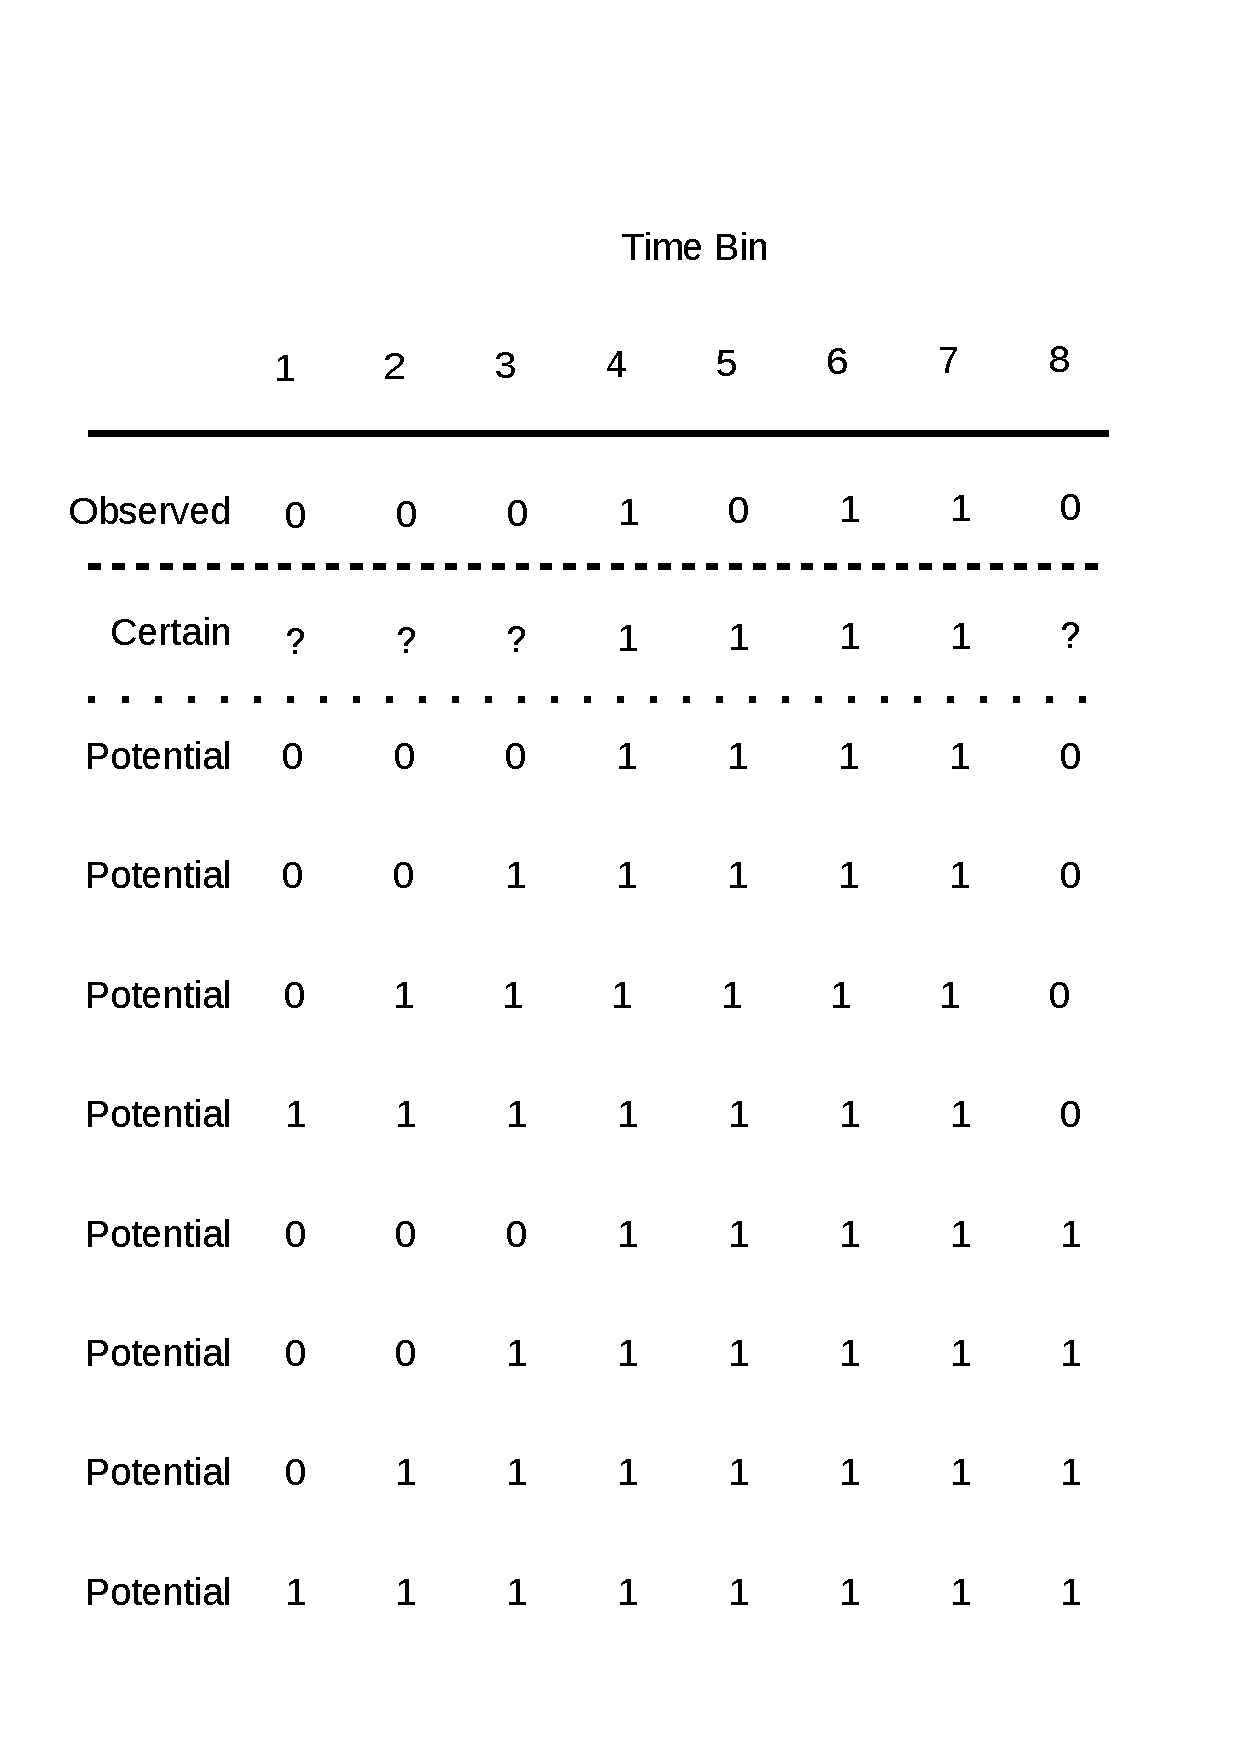
\includegraphics[height=0.4\textheight, width=\textwidth, keepaspectratio=true]{figure/margin}
  \caption[Conceptual figure of all possible occurrence histories for an observed species]{Conceptual figure of all possible occurrence histories for an observed species. The first row represents the observed presence/absence pattern for a single species at eight time points. The second row corresponds to the known aspects of the ``true'' occurrence history of that species. The remaining rows correspond to all possible occurrence histories that are consistent with the observed data. By marginalizing over all possible occurrence histories, the probability of each potential history is estimated. The process of parameter marginalization is described in the text.}
  \label{fig:margin_concept}
\end{figure}


% Stan
%   version 2.9.0
%   marginalize over latent discrete parameters
%     keeping in mind that species HAVE to range through
%     sum of the log probability for all possible configutations
%     along with the sampling probability given those combinations as well
%     see code for implementation? 
%       it is kind of an annoying amount of math to write up

%The combined size of the dataset and large number of parameters (Eqs. \ref{eq:expanded}, \ref{eq:group}, and \ref{eq:prior}), in specific the total number of latent parameters that are the matrix \(z\), means that MCMC based posterior inference is computationally slow. Instead, an approximate Bayesian approach was used: variational inference. A recently developed automatic variational inference algorithm called ``automatic differention variational inference'' (ADVI) is implemented in Stan and is used here \citep{Kucukelbir2015,StanDevelopmentTeam2016}. ADVI assumes that the posterior is Gaussian but still yields a true Bayesian posterior; this assumption is similar to quadratic approximation of the likelihood function commonly used in maximum likelihood based inference \citep{McElreath2016}. The principal limitation of assuming the joint posterior is Gaussian is that the true topology of the log-posterior isn't estimated; this is a particular burden for scale parameters which are bounded to be positive (e.g. standard deviation).
Posterior inference was accomplished using the Hamiltonian Monte Carlo (HMC) routine modified with the No U-Turn Sampler (NUTS) as implemented in the probabilistic programming language Stan CITATION. HMC, which is a gradient based algorithm, is expected to be faster with respect to number of effective samples per Monte Carlo step than the common Gibbs sampling process and is well suited for inference of high dimensional multi-level models such as the one used here. Inference was done using default settings for HMC/NUTS except for the following changes: four chains each run for warm-up length 5000, 5000 post-warm-up samples, and thinned to every fifth sample; initial parameter estimates set to 0; and adapt delta set to 0.9. These settings ensure well mixed chains with good sampling coverage of the estimated log-posteriors.


Of additional concern for posterior inference is the potential of partial identifiable observation parameters \(p_{t = 1}\) and \(p_{t = T}\) \citep{Royle2008}. This issue means that the estimates of sampling probabilities at the ``edges'' of the time series cannot fully be estimated because there are no known ``gaps'' in species occurrence histories that are guaranteed to be filled. Instead, the values of the first and final columns of the ``true'' presence-absence matrix \(z\) for thos observations that do not already have presences in the observed presence-absence matrix \(y\) cannot be estimated \citep{Royle2008}. The hierarchical modeling approach used here helps mitigate this problem by pulling the values of \(p_{t = 1}\) and \(p_{t = T}\) towards the overall mean of \(p\) \citep{Gelman2013d}, and in fact this approach might be more analytically sound than the more ad-hoc approaches that are occasionally used to overcome this hurdle \citep{Royle2008}. Additionally, because \(p_{t = 1}\) and \(p_{t = T}\) are only partially identifiable, estimates of occurrence \(\theta\) and origination \(\phi\) at \(t = 1\) and estimates of \(\theta\), \(\phi\) and survival \(\pi\) at \(t = T\) may suffer from similar edge effects. Again, the hierarchical modeling approach used here may help correct for this reality by drawing these estimates towards the overall means of those parameters.


Finally, after obtaining approximate estimation of the model posterior, model adequacy and quality of fit were assessed using a posterior predictive check \citep{Gelman2013d}. By simulating 100 theoretical data sets from the posterior estimates of the model parameters and the observed covariate information the congruence between predictions made by the model and the observed empirical data can be assessed. These datasets are simulated by starting with the observed states of the presence-absence matrix at \(t = 1\); from there, the time series roll forward as stochastic processes with covariate information given from the empirical observations. Importantly, this is fundamentally different from observing the posterior estimates of the ``true'' presence-absence matrix \(z\). The posterior predictive check used in this study is to compare the observed average number of observations per species to a distribution of simulated averages; if the empirically observed value sits in the middle of the distribution then the model can be considered adequate in reproducing the observed number of occurrences per species. 

%The ADVI assumption of a purely Gaussian posterior limits the utility and accuracy of the posterior predictive checks because parameter estimates do not reflect the true posterior distribution and are instead just an approximation \citep{Gelman2013d}. Because of this, posterior predictive estimates are themselves only approximate checks of model adequacy. The posterior predictive check that is used in this study focuses on mean occurrence and not to any scale parameters that might be most affected by the ADVI assumptions.


Given parameter estimates, diversity and diversification rates are estimated through posterior predictive simulations. Given the observed presence-absence matrix \(y\), estimates of the true presence-absence matrix \(z\) can be simulated and the distribution of possible occurrence histories can be analyzed. This is conceptually similar to marginalization where the probability of each possible occurrence history is estimated (Fig. \ref{fig:margin_concept}), but now these occurrence histories are generated relative to their estimated probabilities.

The posterior distribution of \(z\) gives the estimate of standing diversity \(N^{stand}_{t}\) for all time points as 
\begin{equation}
  N^{stand}_{t} = \sum_{i = 1}^{M} z_{i, t}.
  \label{eq:stand_est}
\end{equation}
Total regional standing diversity can also be partitioned into the standing diversity of each of the functional groups.
%Given estimates of \(N^{stand}\) for all time points, the estimated number of originations \(O_{t}\) is estimated as 
%\begin{equation}
%  O_t = \sum_{i = 1}^{M} z_{i, t} = 1 | z_{i, t - 1} = 0
%  \label{eq:orig_est}
%\end{equation}
%and number of extinctions \(E_{t}\) estimated as
%\begin{equation}
%  E_{t} = \sum_{i = 1}^{M} z_{i, t} = 0 | z_{i, t - 1} = 1.
%  \label{eq:death_est}
%\end{equation}
%Per-capita growth \(D^{rate}\), origination \(O^{rate}\) and extinction \(E^{rate}\) rates are then calculated as
%\begin{equation}
%  \begin{aligned}
%    O^{rate}_{t} &= \frac{O_t}{N^{stand}_{t - 1}} \\
%    E^{rate}_{t} &= \frac{E_t}{N^{stand}_{t - 1}} \\
%    D^{rate}_{t} &= O^{rate}_{t} - E^{rate}_{t}. \\
%  \end{aligned}
%  \label{eq:per_capita_est}
%\end{equation}

% silly transforms using the poisson distribution aren't necessary if you just do the posterior simulations.
% discuss this in the discussion and not this section?

On a final note regarding posterior probabilities and hypothesis tests, when the posterior probability of a hypothesis is 0.80 or greater, I considered that weak evidence in favor of the hypothesis. Similarly, when the posterior probability of 0.90 or greater, I considered that strong evidence in favor of the hypothesis.


\end{document}
